\documentclass[12pt,a4paper]{article}

\usepackage{Act}
\usepackage{listings}

\begin{document}
\input{\detokenize{/home/fenarius/Travail/Cours/Commun/latex/Macros.tex}}

\EP{8}{2022--2023}
\pythonmode

\Exo{Points au scrable}{}

Au Scrabble, chaque lettre possède une valeur et le score d'un mot est la somme des valeurs des lettres qui le compose. Par exemple, la valeur du  mot : 
\begin{center}
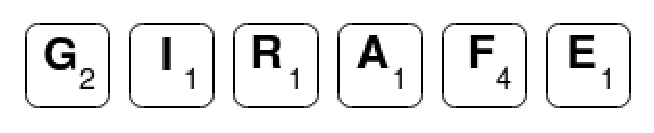
\includegraphics[width=250px]{girafe.eps}
\end{center}
est : $2+1+1+1+4+1=10$. Écrire une fonction  {\tt calcul\_score} qui prend en paramètre une chaîne de caractères {\tt mot} et renvoie sa valeur au Scrabble. Le mot ne doit comporter que les lettres de l'alphabet en majuscules et il peut-être vide. Les valeurs des lettres sont données sur l'illustration suivante :
\begin{center}
    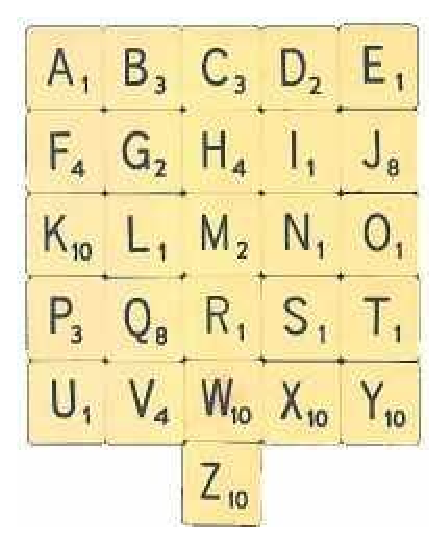
\includegraphics[width=150px]{lettres.eps}
 \end{center}
\textbf{Exemples :}
\begin{lstlisting}
>>> calcul_score("KAYAK")
32
>>> calcul_score("INFORMATIQUE") 
23
>>> calcul_score("")
0
\end{lstlisting}

\vspace{0.2cm}

\Exo{Rectangle en POO}{}

Compléter la classe {\tt Rectangle} en écrivant pour cette classe les méthodes :
\begin{itemize}
\item {\tt aire} qui renvoie la surface du rectangle (largeur fois longueur)
\item {\tt perimetre} qui renvoie le périmètre du rectangle (2 fois longueur plus 2 fois largeur)
\end{itemize}

\begin{lstlisting}
class Rectangle:

    def __init__(self,largeur,longueur):
        self.largeur = largeur
        self.longueur = longueur
    
\end{lstlisting}

Utiliser cette classe et les méthodes pour créer un objet rectangle de dimension 50 sur 15 et afficher son aire et sa surface.
\end{document}
